\section{Αποτελέσματα -- Συζήτηση}

\subsection{Προσομοιώσεις}

\paragraph{} Στην ενότητα αυτή παρουσιάζονται τα αποτελέσματα διαφόρων προσομοιώσεων. Τα
αποτελέσματα εξάγονται από το πρόγραμμα προσομοίωσης με τη μορφή αρχείων κειμένου
\eng{VTK}, τα οποία στη συνέχεια μπορούν να οπτικοποιηθούν και να διερευνηθούν διαδραστικά
μέσω διαφόρων ειδικών προγραμμάτων. Στην παρούσα εργασία, ως πρόγραμμα οπτικοποίησης
χρησιμοποιήθηκε το \eng{ParaView}, που αναπτύσσεται και διανέμεται ως ελεύθερο λογισμικό
από το \eng{Los Alamos National Laboratory}, το \eng{Sandia National Laboratory} και την
εταιρεία \eng{Kitware}. Το \eng{ParaView} τρέχει σε όλα τα ευρέως χρησιμοποιούμενα
λειτουργικά συστήματα (\eng{Unix/Linux, MS Windows, Mac OS X}), διαθέτει αρχιτεκτονική
\eng{client - server} για την οπτικοποίηση δεδομένων που βρίσκονται σε δίκτυο, υποστηρίζει
αρχιτεκτονικές κατανεμημένης επεξεργασίας ενώ δημιουργεί \eng{LOD} (\eng{Level of Detail})
οπτικοποιήσεις για την διατήρηση διαδραστικού αριθμού \eng{FPS} ακόμα και για μεγάλου
όγκου δεδομένα.

% \begin{figure}[]
%   \centering
%   \includegraphics[width=\textwidth]{figures/paraview-interface.png}
%   \caption[Οπτικοποίηση προσομοίωσης] {Οπτικοποίηση προσομοίωσης τσουνάμι \eng{85k}
%     σωματιδίων στο \eng{ParaView}, στιγμιότυπο οθόνης. Αριστερά φαίνεται το ιεραρχικό
%     δένδρο των δεδομένων που οπτικοποιούνται, στη μέση η ανακατασκευή της επιφάνειας του
%     ρευστού σε συνδυασμό με το μοντέλο της ακτογραμμής, ενώ δεξιά οι ώσεις που ασκεί το
%     ρευστό στο επιλεγμένο τμήμα του μοντέλου καθώς και γραφική απεικόνιση αυτών σε
%     ιστόγραμμα.}
%   \label{fig:paraview-interface}
% \end{figure}

\begin{sidewaysfigure}
  \centering
  \includegraphics[width=\textwidth]{figures/paraview-interface.png}
  \caption[Οπτικοποίηση προσομοίωσης] {Οπτικοποίηση προσομοίωσης τσουνάμι \eng{85k}
    σωματιδίων στο \eng{ParaView}, στιγμιότυπο οθόνης. Αριστερά φαίνεται το ιεραρχικό
    δένδρο των δεδομένων που οπτικοποιούνται, στη μέση η ανακατασκευή της επιφάνειας του
    ρευστού σε συνδυασμό με το μοντέλο της ακτογραμμής, ενώ δεξιά οι ώσεις που ασκεί το
    ρευστό στο επιλεγμένο τμήμα του μοντέλου καθώς και γραφική απεικόνιση αυτών σε
    ιστόγραμμα.}
  \label{fig:paraview-interface}
\end{sidewaysfigure}

\paragraph{} Στην εικόνα \ref{fig:paraview-interface} φαίνεται σε στιγμιότυπο οθόνης το
περιβάλλον του \eng{ParaView} κατά την οπτικοποίηση μιας προσομοίωσης \eng{85k}
σωματιδίων. Στην αριστερή στήλη διακρίνεται το δένδρο με τις χρονοσειρές δεδομένων, στο
κορυφαίο επίπεδο του οποίου υπάρχουν το χρωματικό πεδίο (\eng{color\_field}), τα σωματίδια
της προσομοίωσης (\eng{particles}), οι ώσεις του ρευστού προς την ακτογραμμή
(\eng{terrain\_impulses}) και το μοντέλο της ακτογραμμής (\eng{terrain.obj}). Το ίδιο
σύνολο δεδομένων μπορεί να οπτικοποιηθεί ταυτόχρονα με πολλούς τρόπους, σε διάφορα
\eng{RenderViews}. Στο \eng{RenderView2} έχει επιλεγεί η απεικόνιση του μοντέλου της
ακτογραμμής σε γενική άποψη καθώς και της ισοεπιφάνειας του χρωματικού πεδίου, η οποία
δεδομένου ότι το χρωματικό πεδίο αντιπροσωπεύει την αδιάστατη πυκνότητα του ρευστού
αποτελεί μια αποδεκτή προσεγγιστική ανακατασκευή της επιφάνειάς του. Στο \eng{RenderView1}
έχει επιλεγεί η εστιασμένη απεικόνιση τμήματος της ακτογραμμής σε συνδυασμό με τις εντός
του κουτιού επιλογής (\eng{clip}) ώσεις προς αυτήν, οι οποίες είναι χρωματικά διαφορετικές
αναλόγως του μεγέθους τους και αναπαρίστανται σε ιστόγραμμα (\eng{BarChartView1}), όπου
είναι εύκολο να παρατηρηθεί η κατανομή της ορμής στα σωματίδια.

\begin{figure}[h]
  \begin{subfigure}{.5\textwidth}
    \centering
    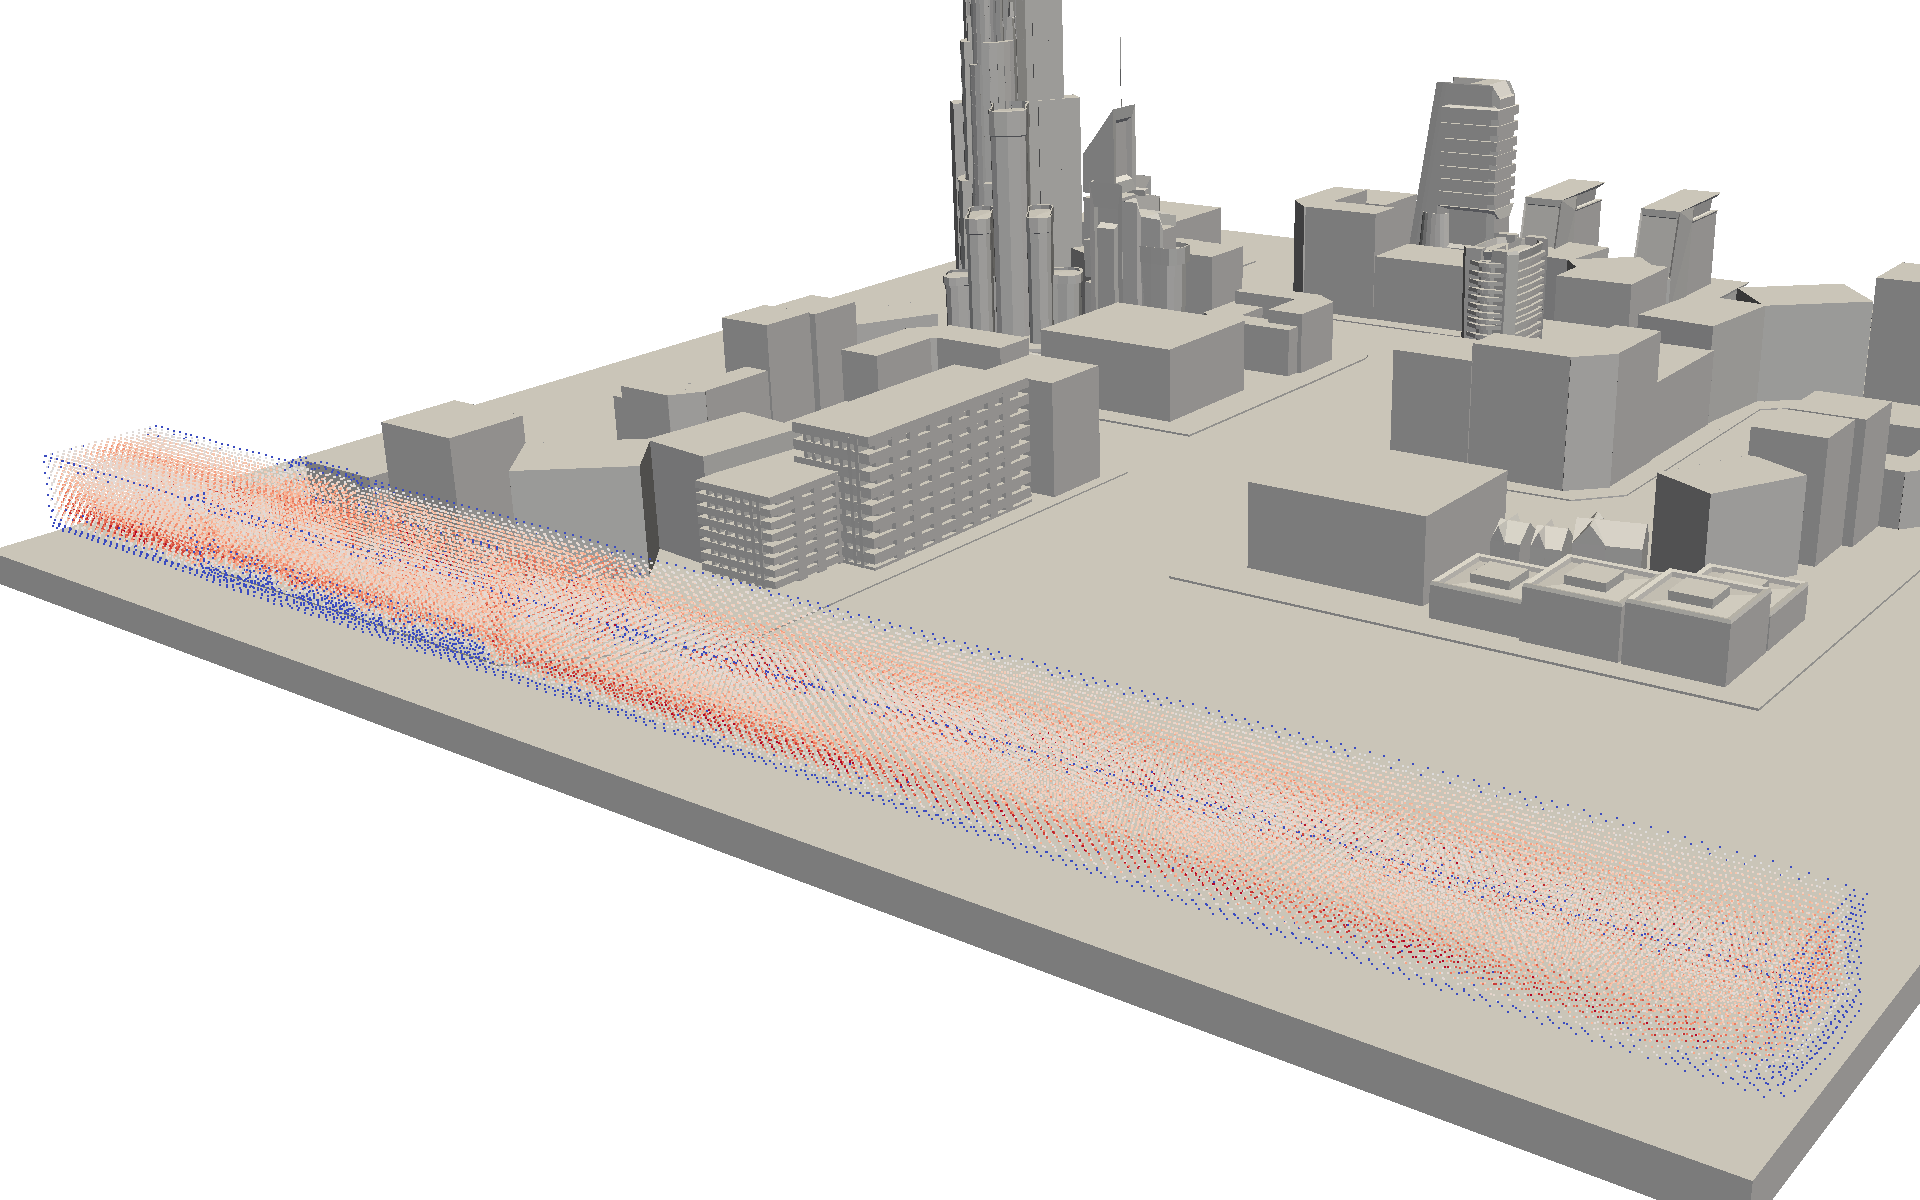
\includegraphics[width=\textwidth]{figures/press-0.png}
  \end{subfigure}
  \begin{subfigure}{.5\textwidth}
    \centering
    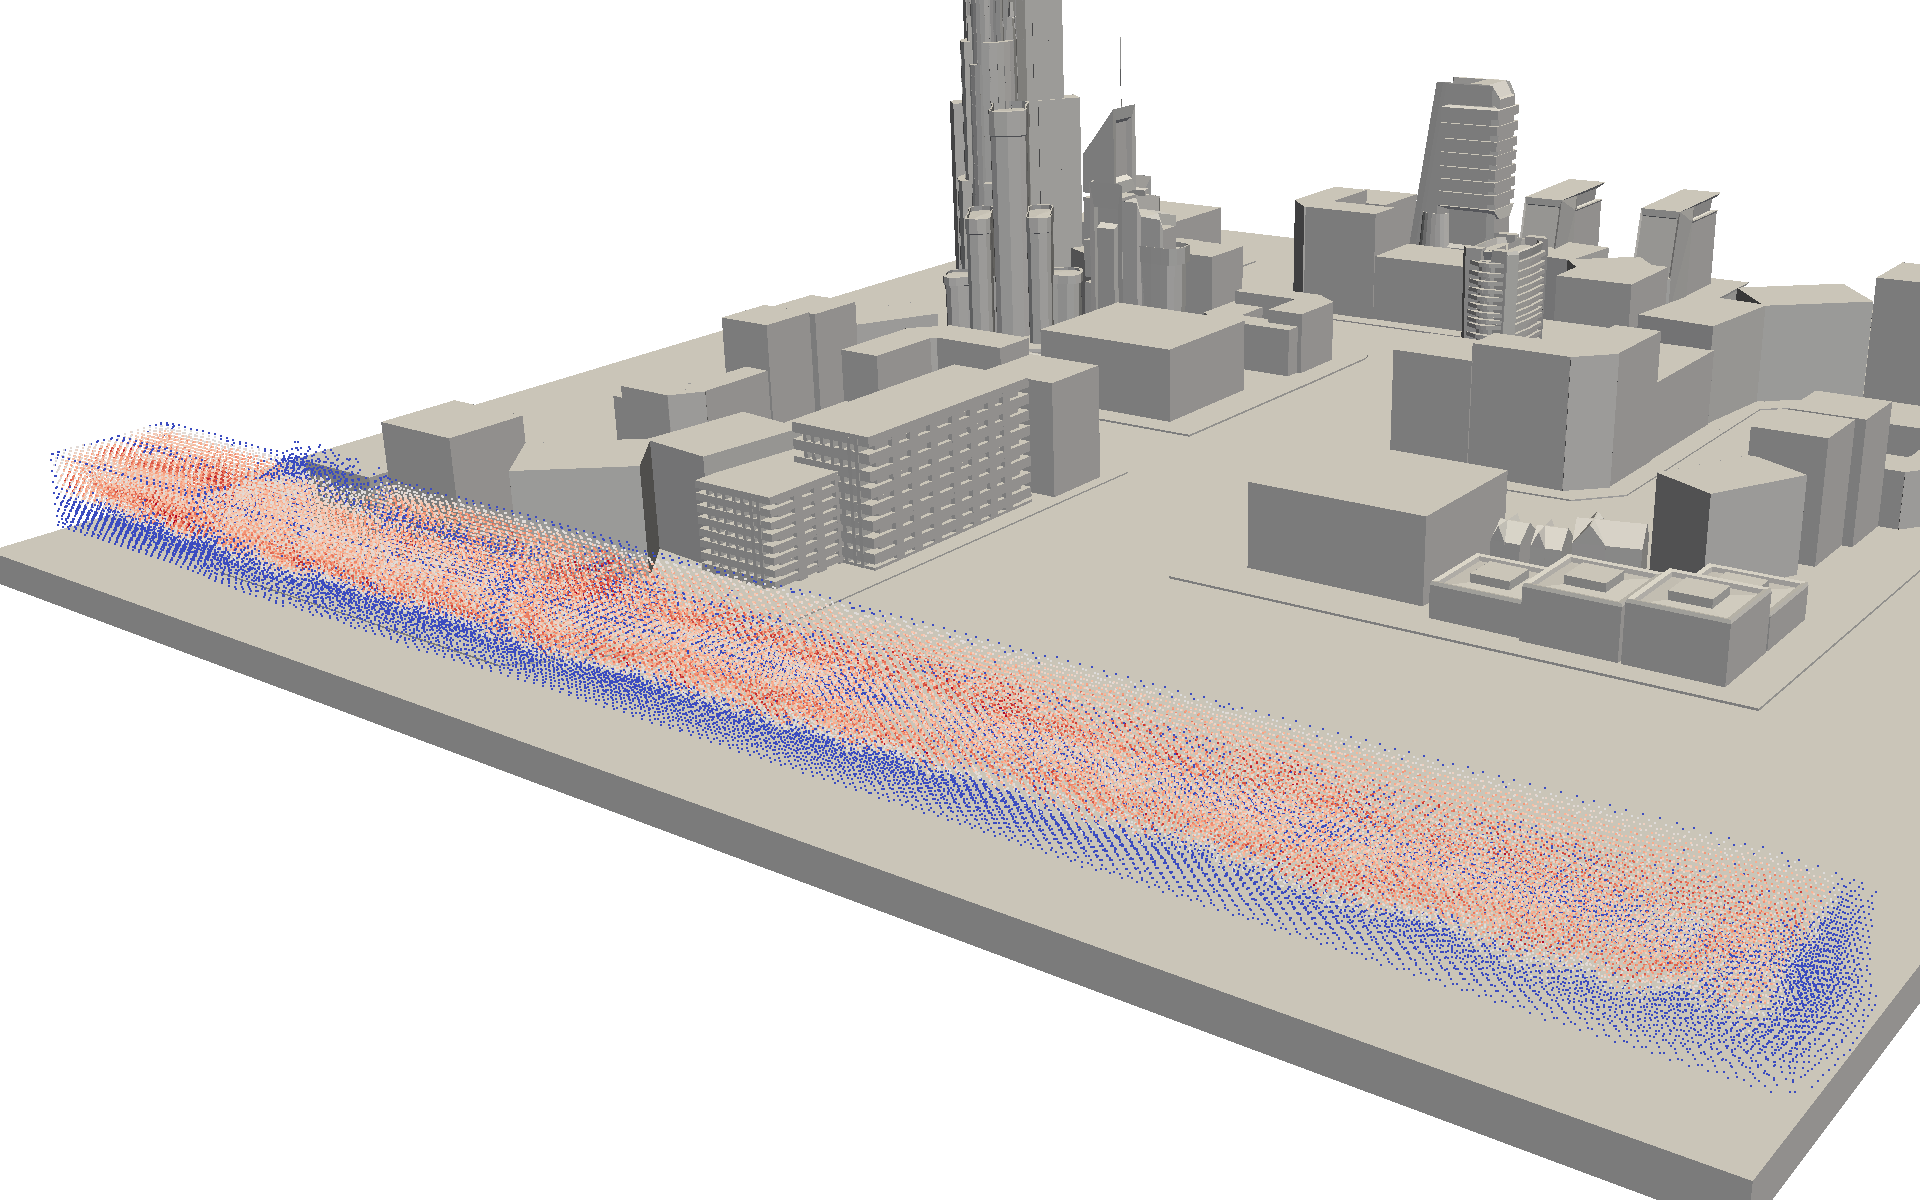
\includegraphics[width=\textwidth]{figures/press-1.png}
  \end{subfigure}
  \begin{subfigure}{.5\textwidth}
    \centering
    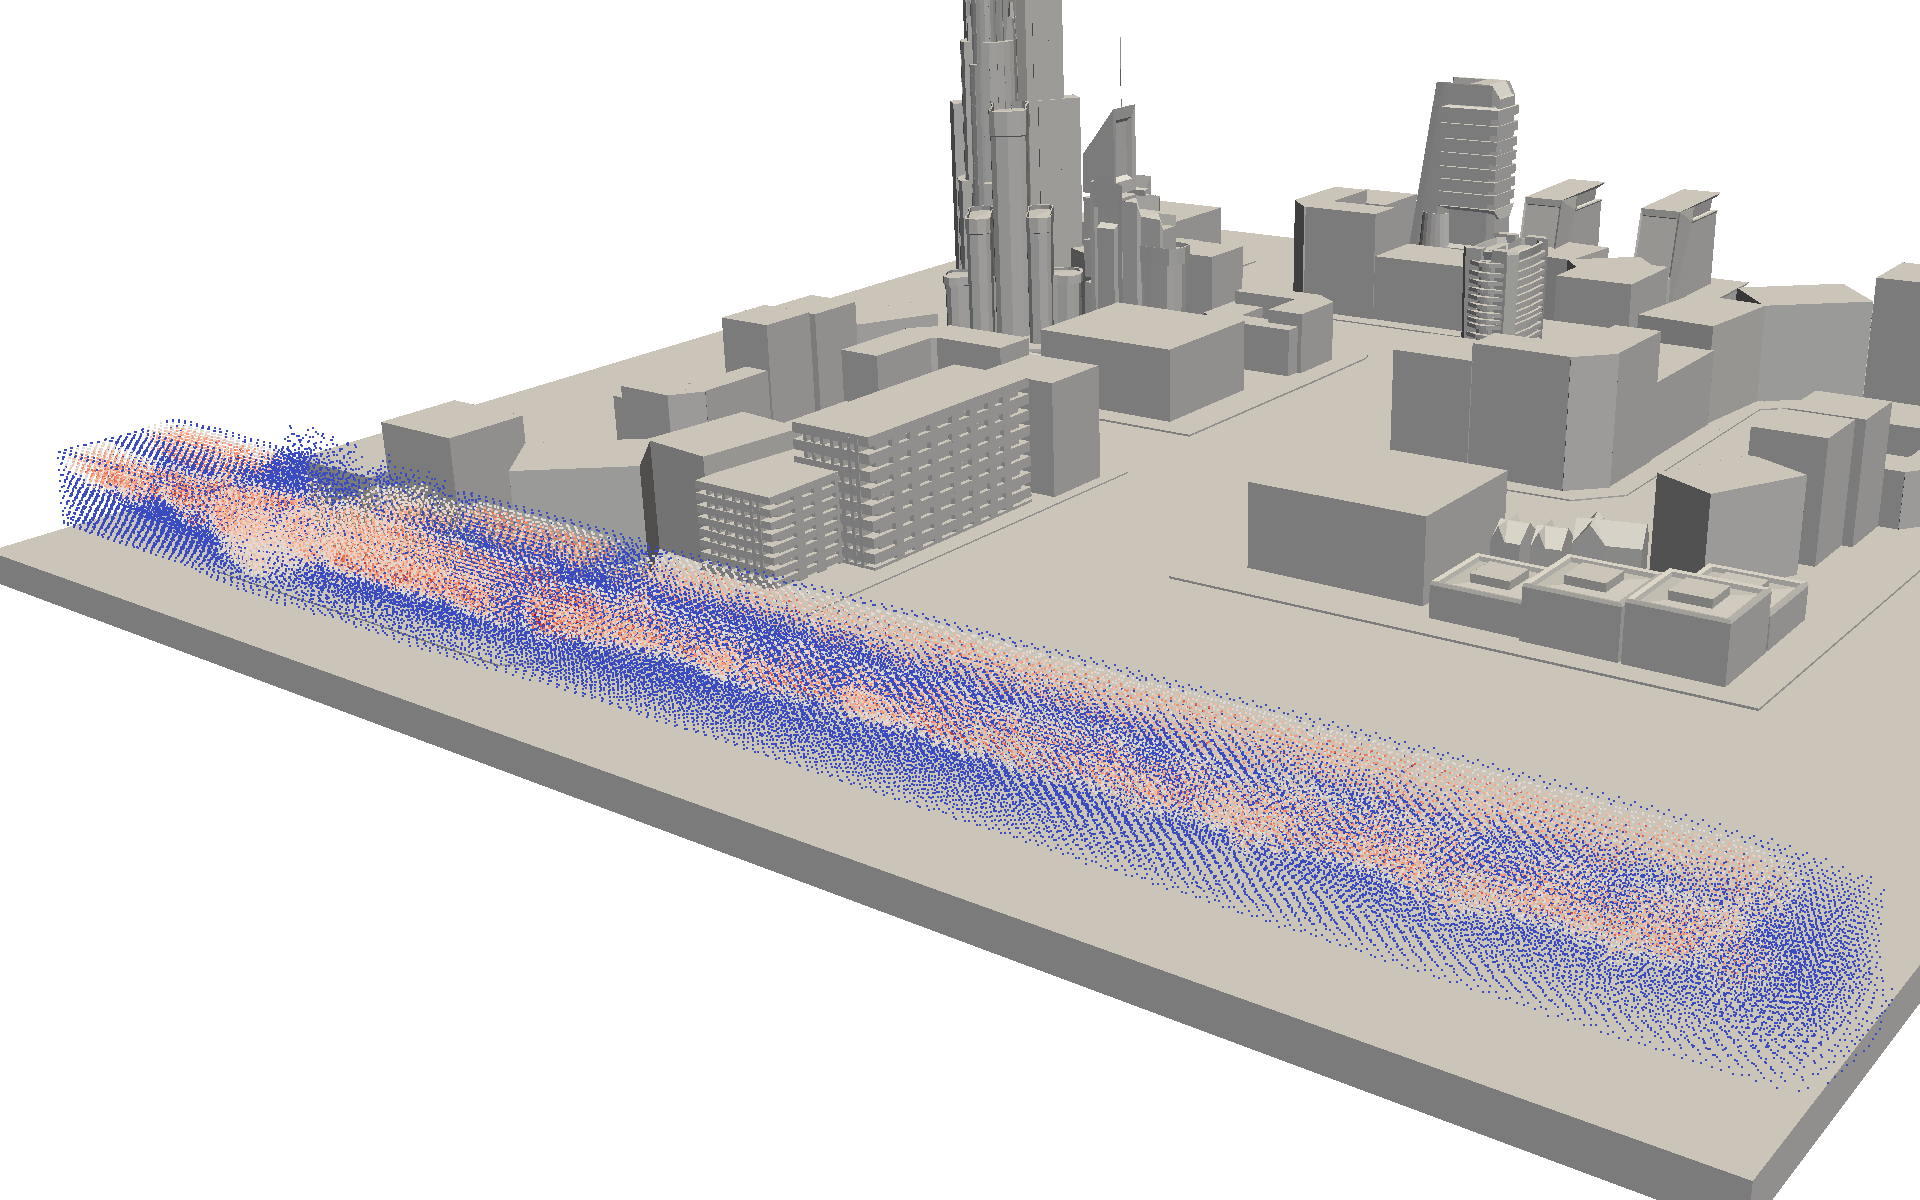
\includegraphics[width=\textwidth]{figures/press-2.png}
  \end{subfigure}
  \begin{subfigure}{.5\textwidth}
    \centering
    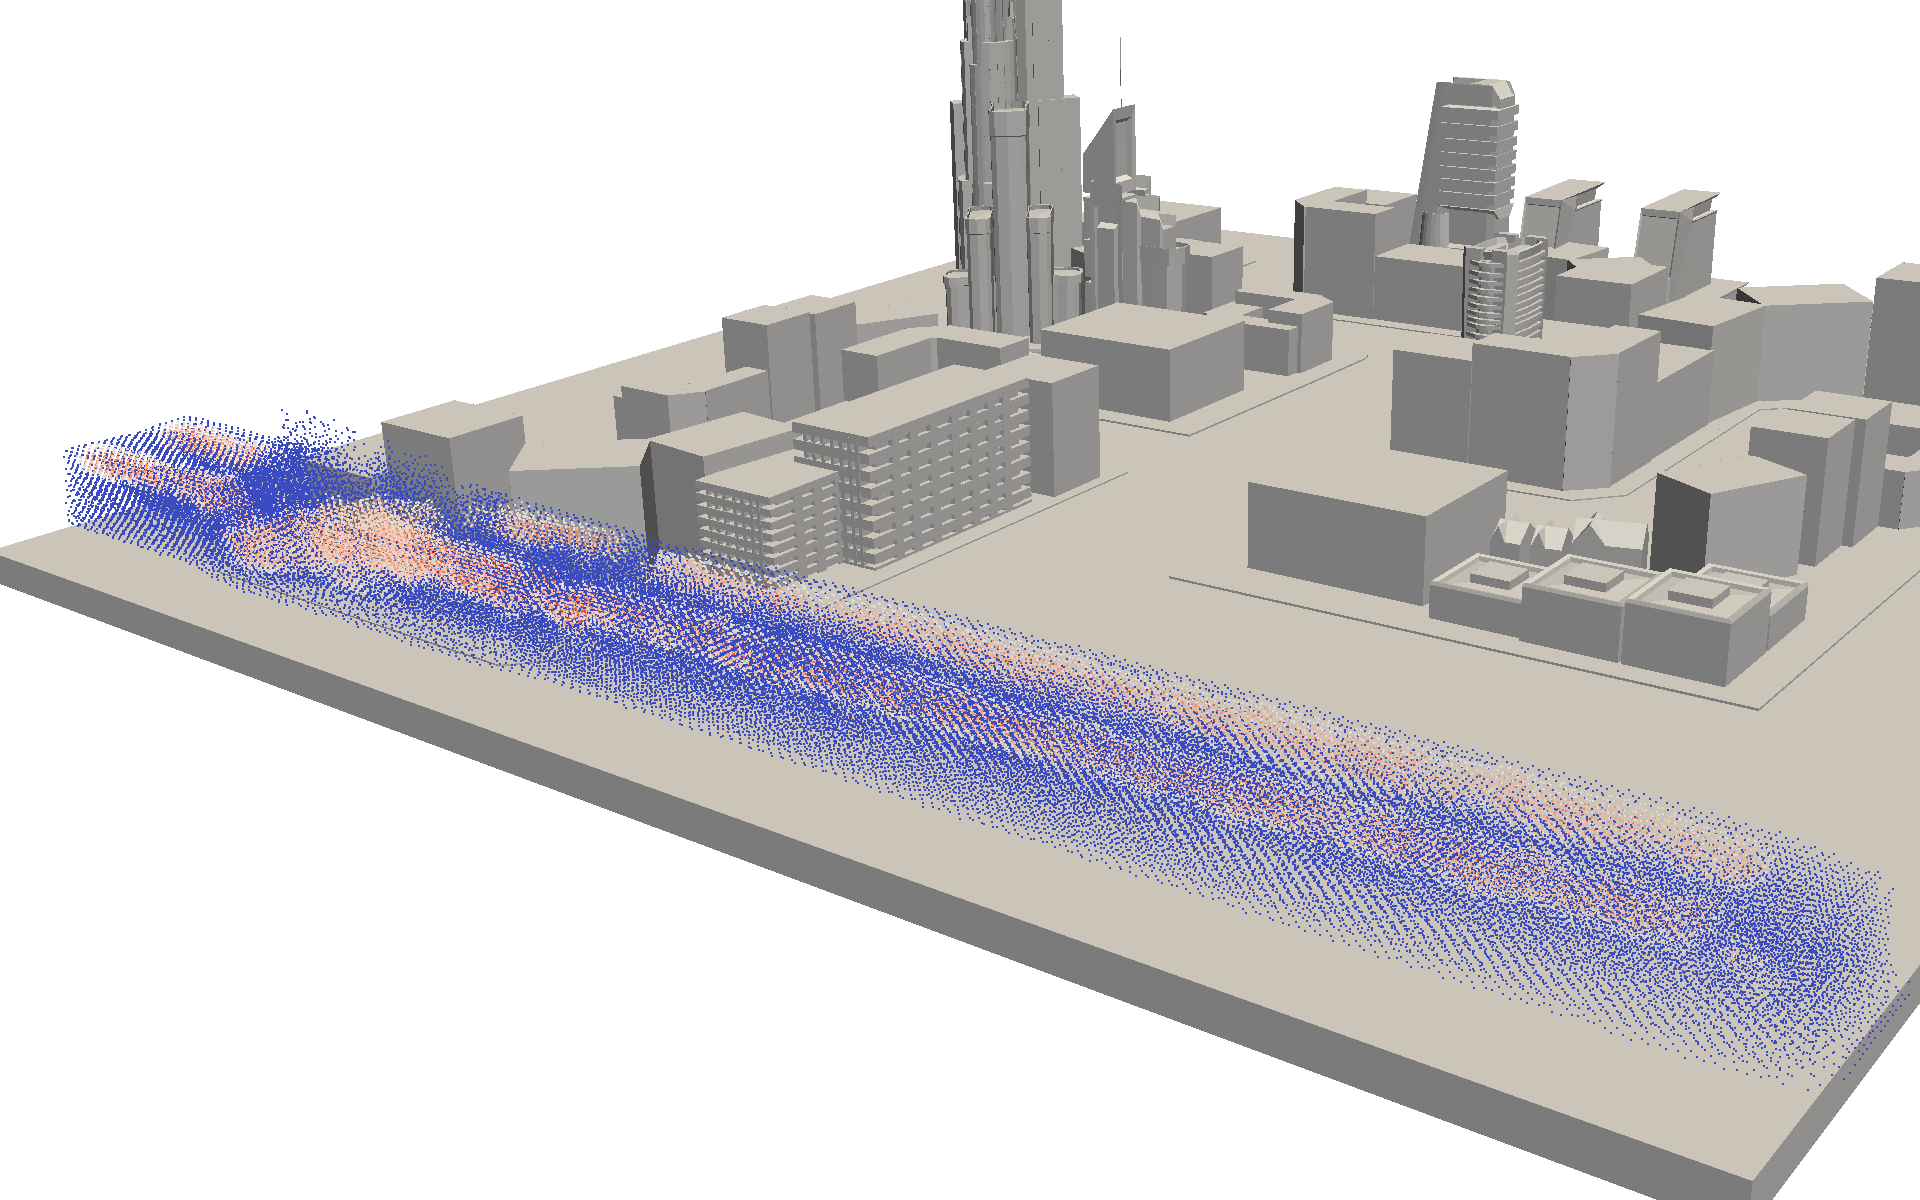
\includegraphics[width=\textwidth]{figures/press-3.png}
  \end{subfigure}
  \begin{subfigure}{.5\textwidth}
    \centering
    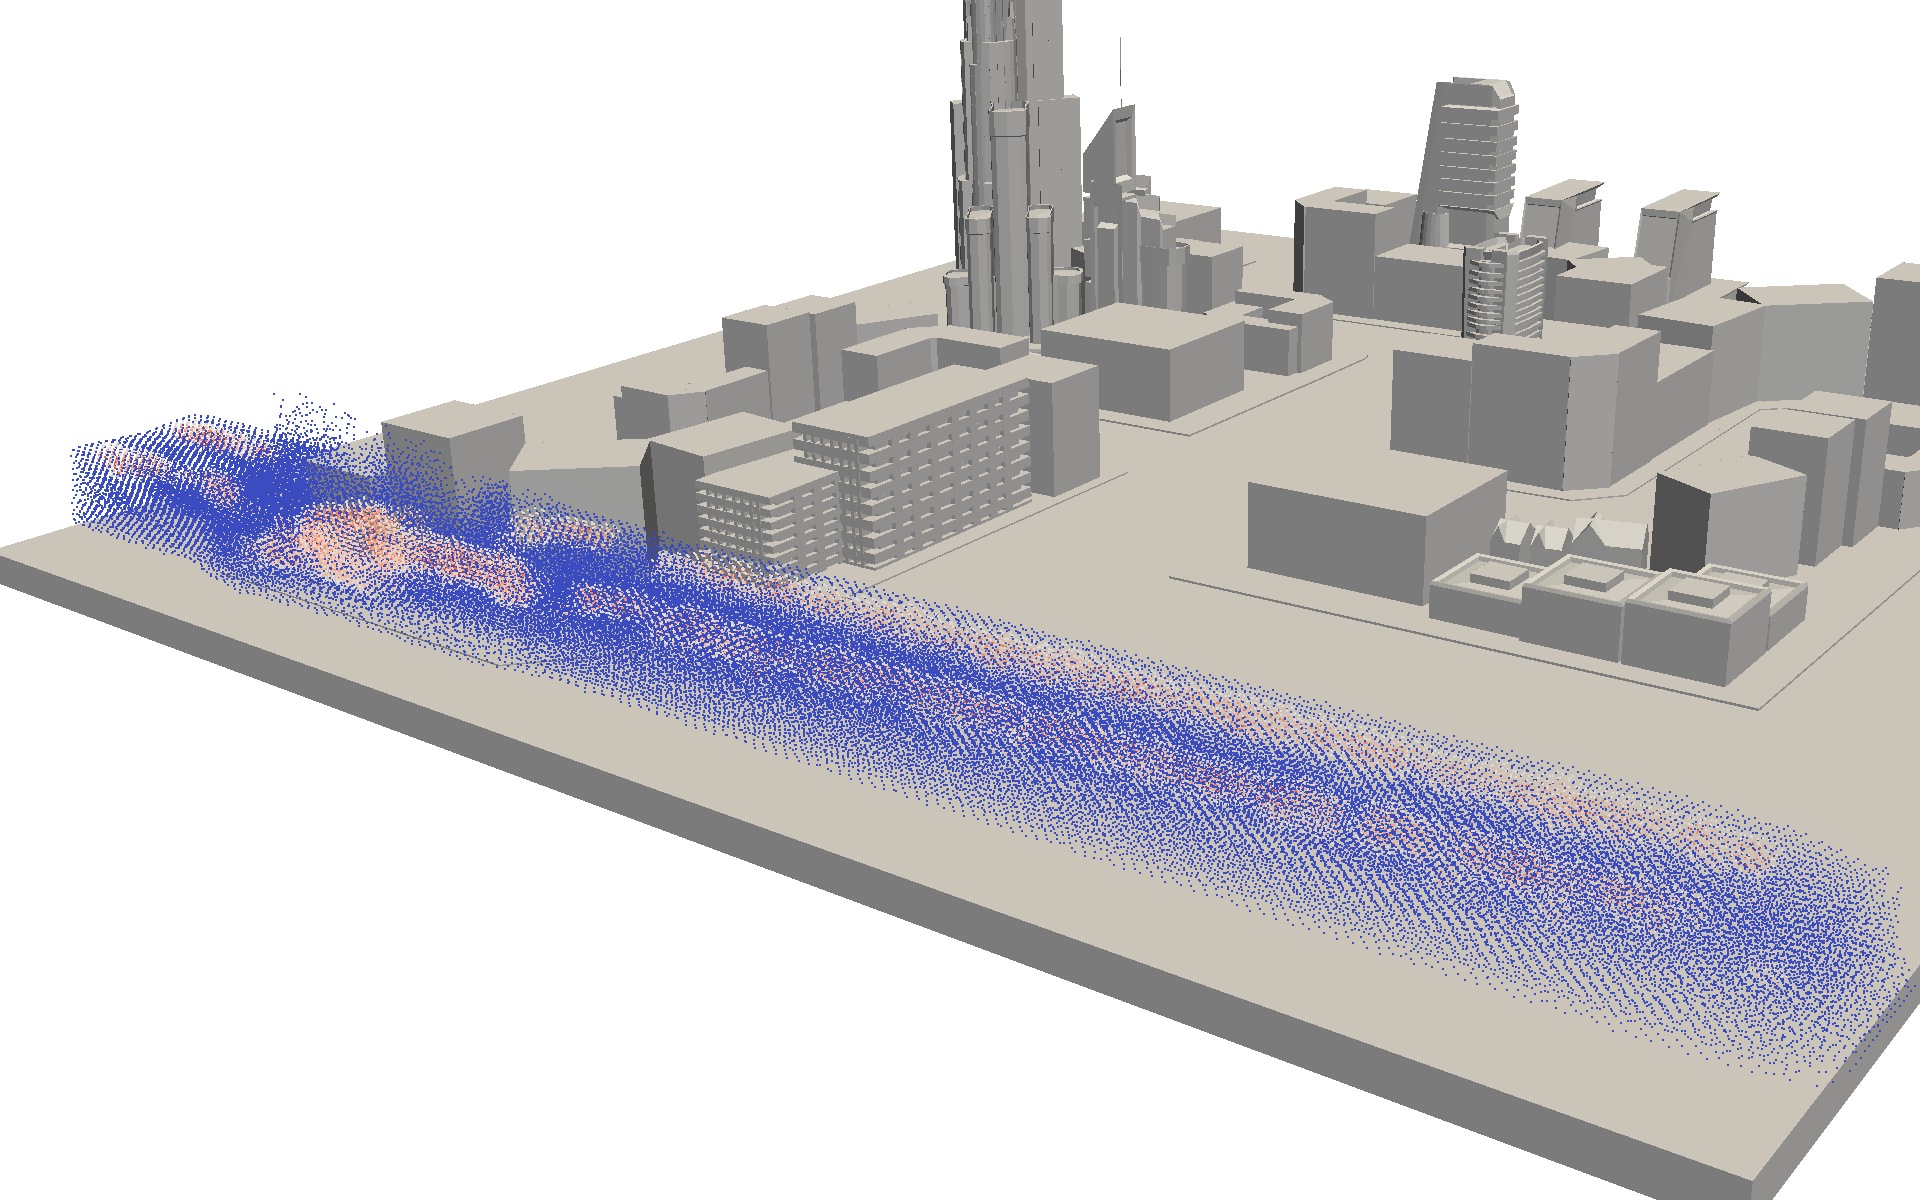
\includegraphics[width=\textwidth]{figures/press-4.png}
  \end{subfigure}
  \begin{subfigure}{.5\textwidth}
    \centering
    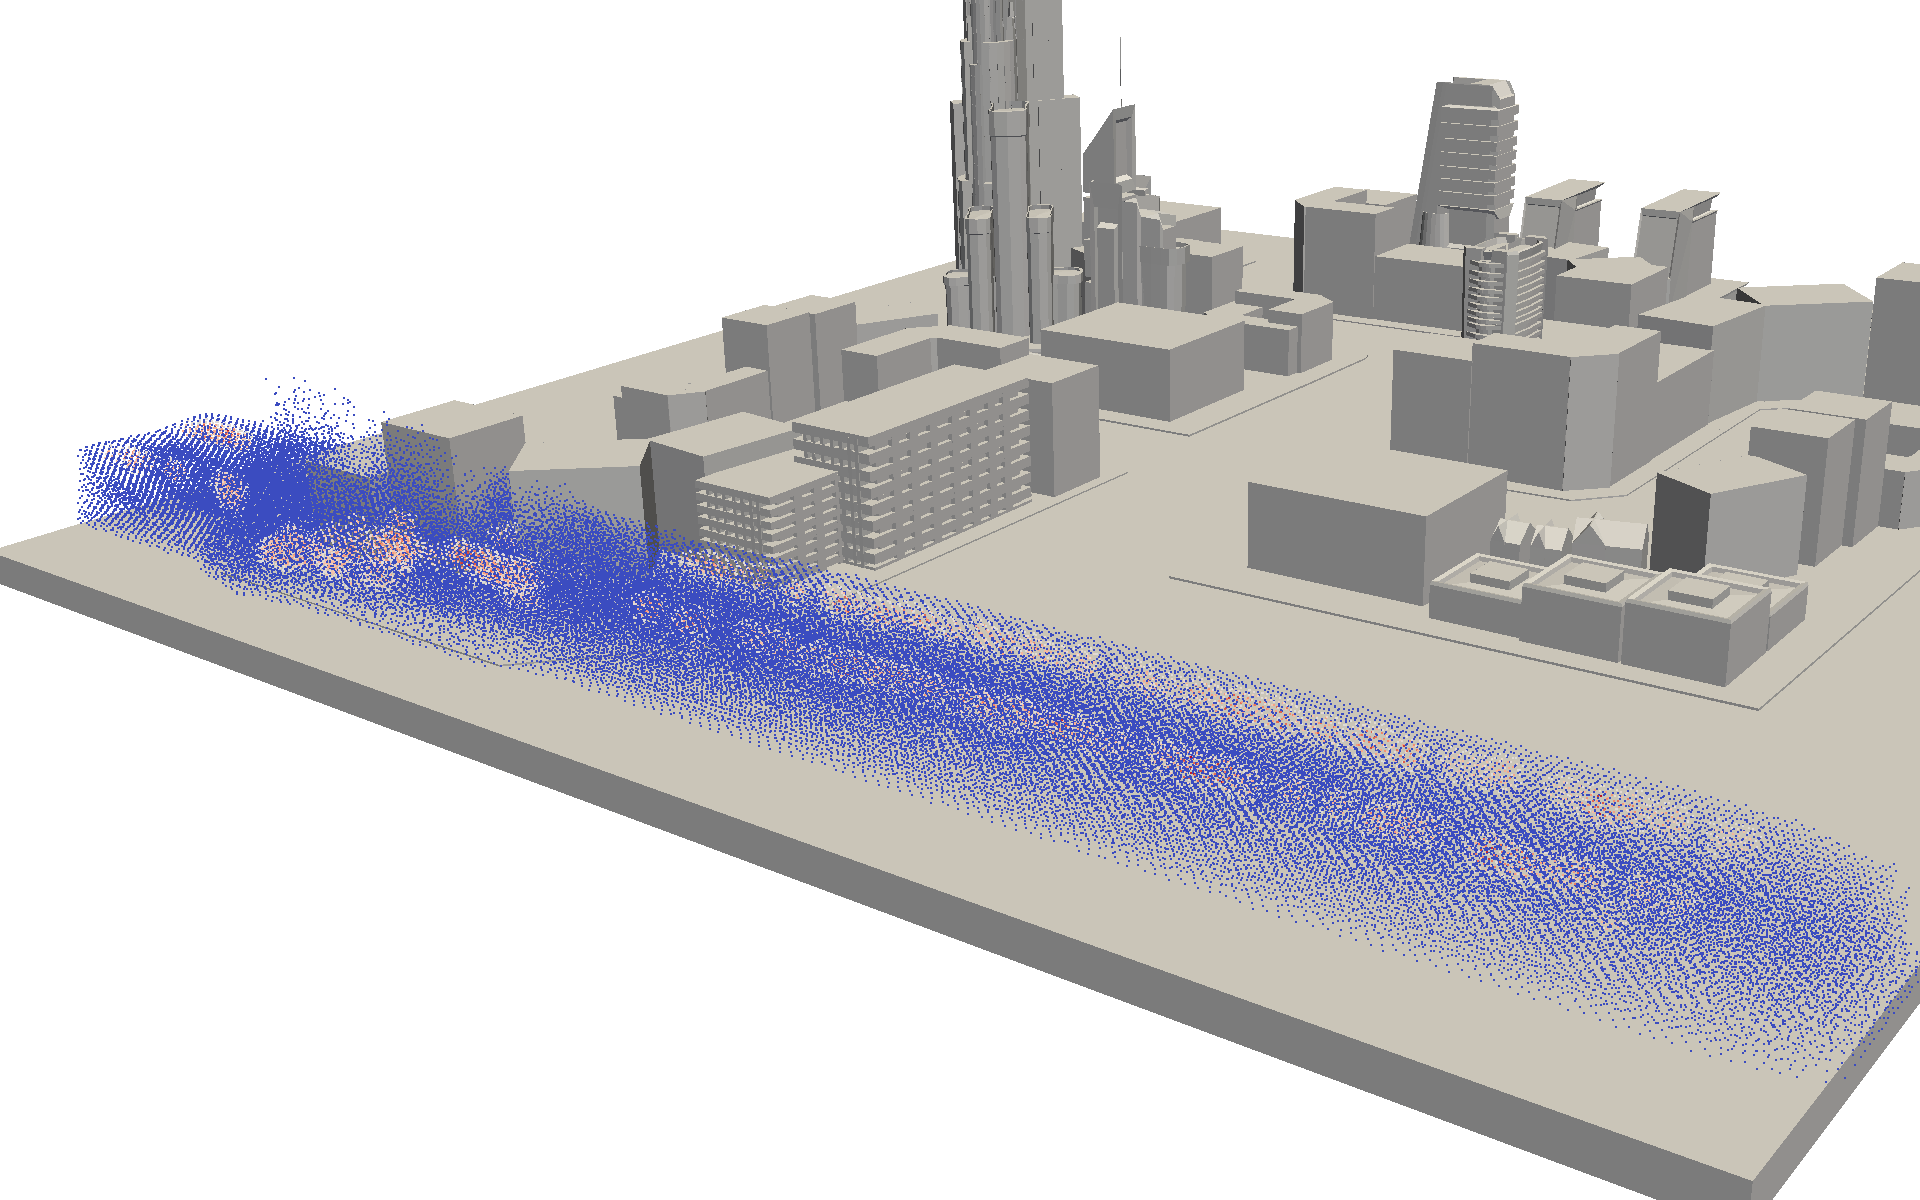
\includegraphics[width=\textwidth]{figures/press-5.png}
  \end{subfigure}
  \caption[Διάδοση δυνάμεων πίεσης]{Διαδοχικά στιγμιότυπα προσομοίωσης όπου αποτυπώνεται η
    διάδοση της ώσης του εδάφους στη υπερκείμενη στήλη νερού με τη μορφή δυνάμεων
    πίεσης. Τα σωματίδια της προσομοίωσης αναπαρίστανται με σημεία χρωματισμένα σύμφωνα με
    το μέτρο των δυνάμεων πίεσης που ασκούνται στο καθένα (θερμότητα χρώματος ανάλογη του
    μέτρου της δύναμης).}
  \label{fig:pressure-forces}
\end{figure}

\paragraph{} Όσον αφορά τις δυνάμεις που ασκούνται εντός του ρευστού, στις εικόνες
\ref{fig:pressure-forces} και \ref{fig:viscosity-forces} απεικονίζονται σε διαδοχικά
στιγμιότυπα τα σωματίδια της ίδιας προσομοίωσης, χρωματικά κωδικοποιημένα με βάση τις
δυνάμεις που ασκούνται σε αυτά λόγω πίεσης και ιξώδους αντίστοιχα. Το τσουνάμι
αναπαρίσταται σαν ένας όγκος νερού που εισβάλλει στην ακτογραμμή με μια σταθερή
ταχύτητα. Η προσέγγιση αυτή βρίσκεται αρκετά κοντά στην πραγματικότητα, δεδομένου οτι τα
τσουνάμι εκδηλώνονται ως μερικές επαναλαμβανόμενες, ορμητικές παλλίροιες της θάλασσας, με
μεγάλους όγκους νερού να ρέουν προς την ενδοχώρα. Στην εικόνα \ref{fig:pressure-forces}
παρατηρείται η διάδοση της ώσης του εδάφους στα αρχικά στάδια της προσομοίωσης μέσω
δυνάμεων πίεσης στη σχετικά άθικτη ακόμα υδάτινη στήλη (θερμότητα χρώματος ανάλογη του
μέτρου της δύναμης). Παρόμοια χρωματισμένες στην εικόνα \ref{fig:viscosity-forces}
διακρίνονται οι δυνάμεις ιξώδους, που οφείλονται στη διαφορά ταχύτητας μεταξύ γειτονικών
σωματιδίων και ως εκ τούτου είναι ισχυρές κατά την πρόσκρουση του ρευστού σε εμπόδια, όπου
τμήματά του αλλάζούν ταχύτητα σε σχέση με τα κοντινά τους. Στην εικόνα \ref{fig:samples}
τα σωματίδια κωδικοποιούνται χρωματικά σύμφωνα με το πλήθος γειτονικών σωματιδίων εντός
της ακτίνας εξομάλυνσης της προσομοίωσης. Όπως φαίνεται, λόγω της φύσης της προσομοίωσης
(ροή σε ανοιχτό χώρο με πολύπλοκα όρια) το ρευστό διαθέτει υψηλό λόγο επιφάνειας προς
όγκο, με αποτέλεσμα μεγάλο του μέρος να υποφέρει από υποδειγματοληψία. Για το λόγο αυτό
υιο\-θε\-τή\-θη\-καν (όπως αναλύθηκε και στην παράγραφο \ref{sssec:fluid-init})
γεωμετρικοί περιορισμοί μεταξύ των σωματιδίων για την αναπλήρωση της χαμένης πληροφορίας.

\begin{figure}[h]
  \begin{subfigure}{.5\textwidth}
    \centering
    \includegraphics[width=\textwidth]{figures/visc-0.png}
  \end{subfigure}
  \begin{subfigure}{.5\textwidth}
    \centering
    \includegraphics[width=\textwidth]{figures/visc-1.png}
  \end{subfigure}
  \begin{subfigure}{.5\textwidth}
    \centering
    \includegraphics[width=\textwidth]{figures/visc-2.png}
  \end{subfigure}
  \begin{subfigure}{.5\textwidth}
    \centering
    \includegraphics[width=\textwidth]{figures/visc-3.png}
  \end{subfigure}
  \caption[Δυνάμεις ιξώδους]{Διαδοχικά στιγμιότυπα προσομοίωσης όπου αποτυπώνεται
    χρωματικά στα σωματίδια το μέτρο της δύναμης που τους ασκείται λόγω ιξώδους του
    ρευστού. Η δύναμη του ιξώδους είναι ανάλογη της διαφοράς ταχύτητας μεταξύ γειτονικών
    σωματιδίων, και λόγω αυτού έχουν σημαντικό μέγεθος στις προσκρούσεις με εμπόδια,
    δεδομένης της απότομης αλλαγής ταχύτητας τμήματος του ρευστού (θερμότητα χρώματος
    ανάλογη του μέτρου της δύναμης).}
  \label{fig:viscosity-forces}
\end{figure}

\begin{figure}[h]
  \centering
  \includegraphics[width=\textwidth]{figures/samples.png}
  \caption[Απεικόνιση γειτονικών σωματιδίων] {Στιγμιότυπο προσομοίωσης όπου φαίνεται
    χρωματικά κωδικοποιημένος ο αριθμός των δειγμάτων (γειτονικών σωματιδίων) που
    διατίθενται για την εκτίμηση των ιδιοτήτων του ρευστού (διακύμανση από σκούρο μπλε
    μέχρι έντονο κόκκινο, 0 έως 52 δείγματα αντίστοιχα στην παρούσα περίπτωση). Λόγω της
    φύσης της προσομοίωσης (ροή σε ανοιχτό χώρο) είναι φανερή η έλλειψη ικανοποιητικού
    αριθμού δειγμάτων σε μεγάλο τμήμα του ρευστού, που οδήγησε και στην υιοθέτηση
    στοιχείων από \eng{PBD} (παράγραφος \ref{sssec:fluid-init}, \cite{Muller2007109,
      macklin2013position}).}
  \label{fig:samples}
\end{figure}

\begin{figure}[h]
  \begin{subfigure}{.5\textwidth}
    \centering
    \includegraphics[width=\textwidth]{figures/impulses-0.png}
  \end{subfigure}
  \begin{subfigure}{.5\textwidth}
    \centering
    \includegraphics[width=\textwidth]{figures/impulses-1.png}
  \end{subfigure}
  \begin{subfigure}{.5\textwidth}
    \centering
    \includegraphics[width=\textwidth]{figures/impulses-2.png}
  \end{subfigure}
  \begin{subfigure}{.5\textwidth}
    \centering
    \includegraphics[width=\textwidth]{figures/impulses-3.png}
  \end{subfigure}
  \caption[Ώσεις στην ακτογραμμή]{Διάφορα στιγμιότυπα προσομοίωσης όπου αποτυπώνεται
    χρωματικά στην ακτογραμμή το μέτρο της ώσης που ασκείται από τα σωματίδια του ρευστού
    κατά την εξέλιξη του τσουνάμι (θερμότητα χρώματος ανάλογη του μέτρου της ώσης).}
  \label{fig:impulses}
\end{figure}

\subsection{Συμπεράσματα -- Μελλοντικές επεκτάσεις}
\paragraph{} 

\begin{figure}[h]
  \begin{subfigure}{.5\textwidth}
    \centering
    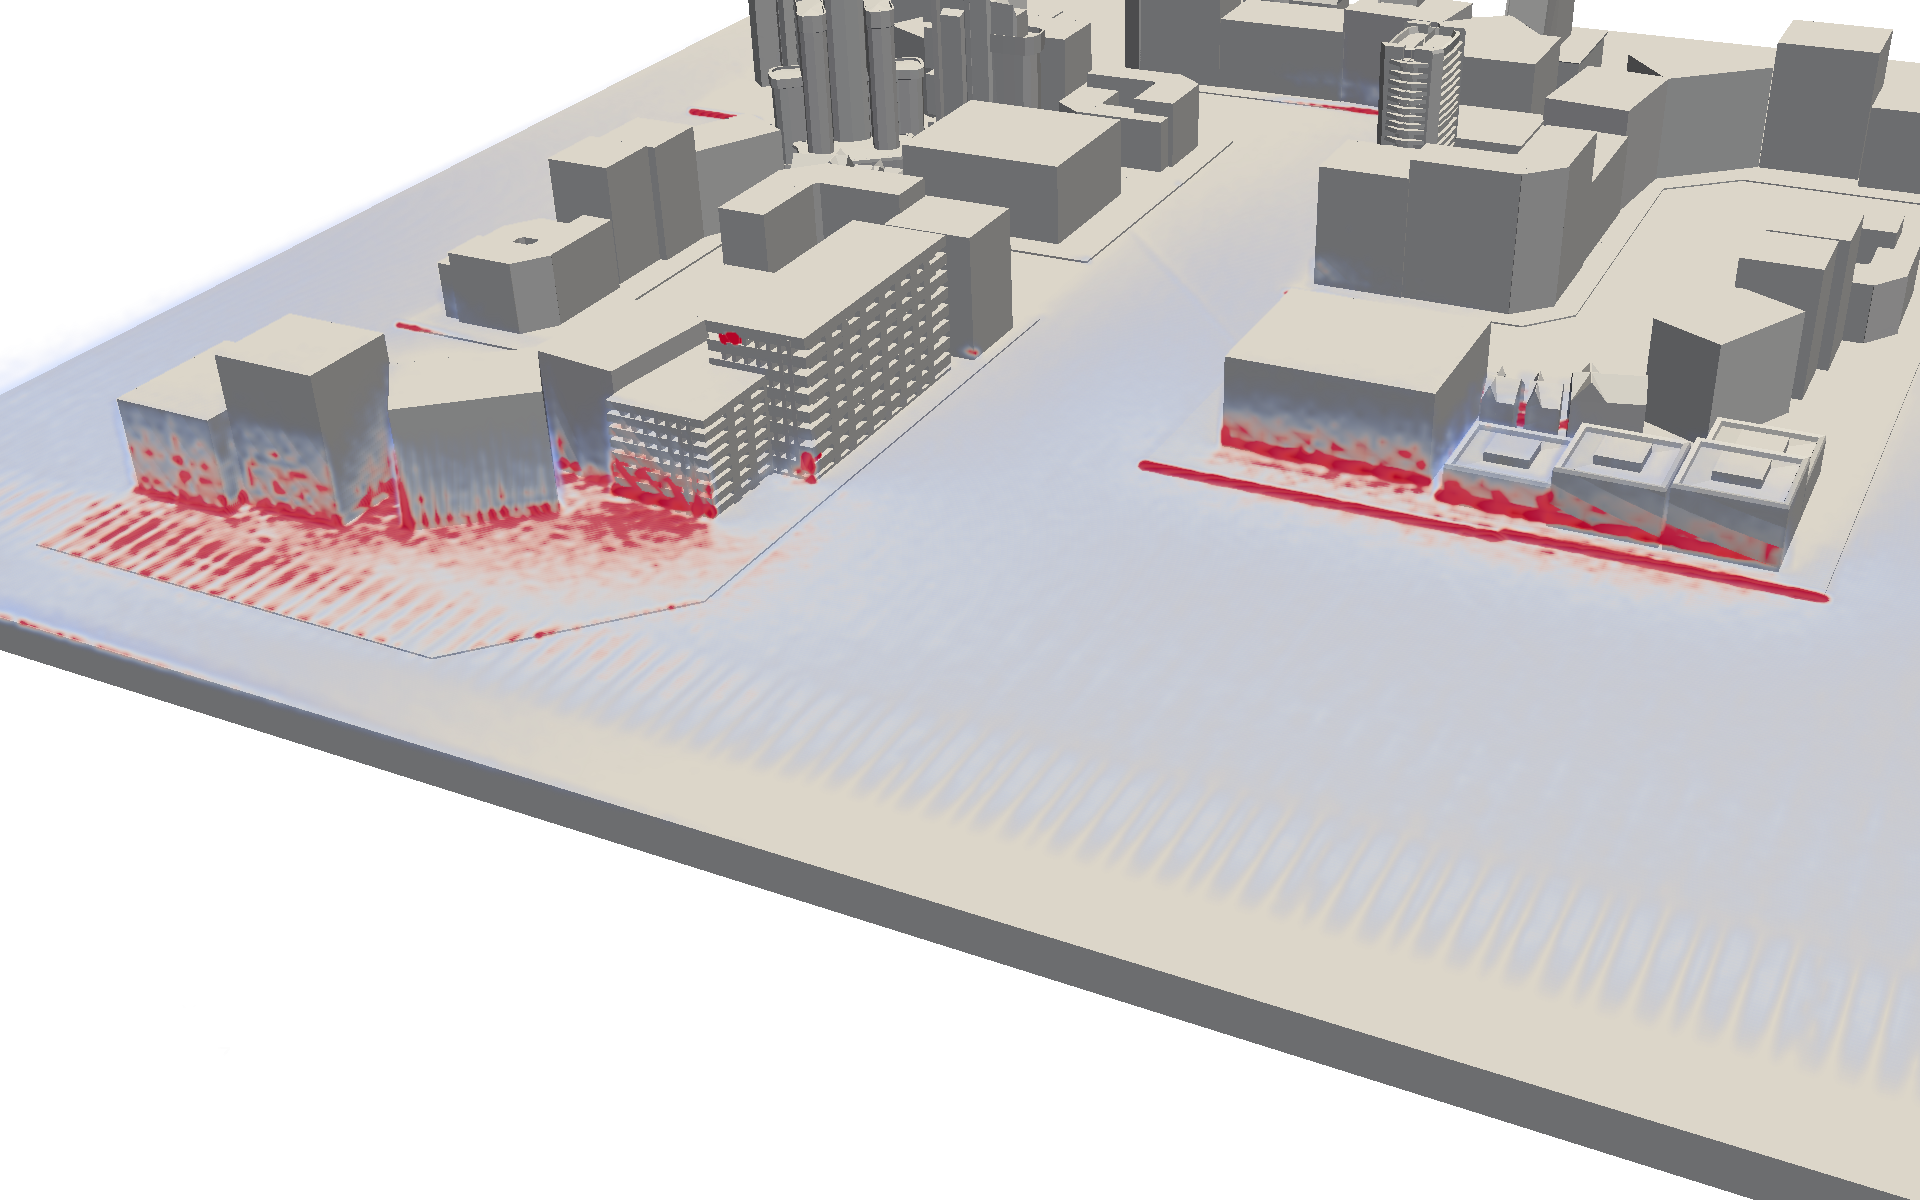
\includegraphics[width=\textwidth]{figures/impulse-heatmap-0.png}
  \end{subfigure}
  \begin{subfigure}{.5\textwidth}
    \centering
    \includegraphics[width=\textwidth]{figures/impulse-heatmap-1.png}
  \end{subfigure}
  \begin{subfigure}{\textwidth}
    \centering
    \includegraphics[width=\textwidth]{figures/impulse-heatmap-2.png}
  \end{subfigure}
  \caption[\eng{Heatmap} ώσεων στην ακτογραμμή]{\eng{Heatmap} των ώσεων του ρευστού προς
    την ακτογραμμή καθ' όλη την εξέλιξη του κύματος, σε τρία διαφορετικά μοντέλα
    πόλης. Επιβεβαιώνεται οτι το μεγαλύτερο μέρος της ενέργειας του κύματος απορροφάται
    από από τα πρώτα εμπόδια που αυτό συναντά, φαινόμενο που έχει δειχθεί τόσο σε
    καταγραφές πραγματικών περιστατικών, όσο και στη βιβλιογραφία.}
  \label{fig:impulse-fields}
\end{figure}

%%% Local Variables:
%%% mode: latex
%%% TeX-master: "report"
%%% End:
